\chapter{How \textsc{Becca}'s feature extractor works}
\label{perceiver_chapter}

This appendix provides enough mathematical detail to fully describe the implementation of the feature extractor. Appendix~\ref{actor_chapter} contains a detailed description of the reinforcement learner.

\textsc{Becca} extracts features by greedily gathering commonly co-active inputs. (See Figure~\ref{becca_feature_extractor}.)  \textsc{Becca} requires no prior knowledge about the environment it is in, the nature of the experiences it is likely to have, or the sensors that provide its input data. The one constraint it places on the world is that its reward and inputs be real valued. Primitives require a small amount of additional engineering: they must be real valued between zero and one. 

\begin{figure}
\centering 
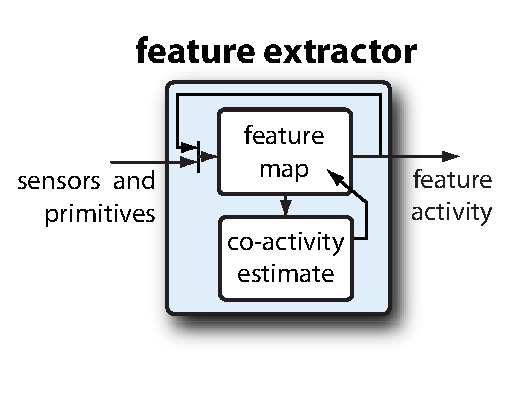
\includegraphics[height=7cm]{figs/becca_feature_extractor.eps}
\caption{Block diagram of \textsc{Becca}'s feature extractor.}
\label{becca_feature_extractor}
\end{figure}

There are several user-selected constants that modify the function of the feature extractor. In the following description, they will be identified as $C_x$ where they subscript provides a unique identifier. They default values for these constants in the current version are listed in table~\ref{perceiver_constants}. 

\section{Input conditioning}
\textsc{Becca} interprets each input as a fuzzy binary value, indicating the degree of presence of an attribute or the degree of activation of a sensor. At each time step, $t$, it receives an array of raw sensor inputs, $\hat{\mathbf{s}}$. The input value $\hat{s}_k$ from each sensor channel $k$ must be mapped to the interval $[0,1]$ to facilitate its interpretation as a graded binary value. This is done adaptively. The mean, $\hat{s}_{k\mu}$, and typical deviation, $\hat{s}_{k\epsilon}$, is estimated incrementally by these formulas:

\begin{eqnarray}
\rho_s &=& C_{sdr} + \frac{C_{sut}}{ t + C_{sut}}\\
s_{k \mu_{t+1}} &=& s_{k \mu_t } (1 - \rho_s)  + \hat{s}_k  \rho_s \\
s_{k \epsilon_{t+1}} &=& s_{k \epsilon_t}  (1 - \rho_s)  + |\hat{s}_k - s_{k \mu_{t+1}}| \rho_s 
\end{eqnarray}

$\rho_s$ here is an update rate that is a function of the agent's age, $t$, the sensor distribution update rate, $C_{sdr}$, and the sensor update time constant, $C_{sut}$. At $t=0$ the value of $s_{k \mu}$ is initialized to $C_{sim}$ and the value of $s_{k \epsilon}$ is initialized to $C_{sid}$. When the agent is very young, the estimates of the mean and deviation change quickly, adapting to the input distributions observed. The adaptation rate slows over time, reflecting increased confidence in the estimates' accuracy.

Using its mean and deviation, each channel is transformed to a roughly zero-mean signal with this relation:

\begin{equation}
s_k = g \left (\frac{\hat{s}_k - s_{k \mu} }{2 s_{k \epsilon}} \right )
\end{equation}

where $g(\cdot)$ is a function that maps the interval $[0, \infty)$ onto $[0,1)$ and the interval $(-\infty,0]$ onto $(-1,0]$:

\begin{equation}
g(x) = 1 - \frac{1}{x + 1} 
\label{inf_to_one_map}
\end{equation}

It's inverse function, $g^\prime(\cdot)$ performs the reverse mapping:

\begin{equation}
g^{-1}(x) = \frac{1}{x} - 1
\label{one_to_inf_map}
\end{equation}

Each of the resulting sensor channels lies on the interval $(-1,1)$. Each channel is then split and rectified into its positive and negative portions, $s_k^+$ and $s_k^-$. This results in a conditioned array of sensor channels, $\mathbf{s}$, that has twice the number of input channels originally passed to the agent.

Primitives are not subject to this process. They have been pre-engineered for compatibility with \textsc{Becca} (i.e. they are hacks) and are already on $[0, 1]$.

\section{Co-activity based feature extraction}
The extraction of new features is driven by how often each input channel is co-active with each of the other channels. The process of feature extraction finds sets of input channels that tend to be mutually co-active. Sets of commonly co-occurring inputs represent pieces of observed structure in the world.

When two channels are co-active, both have a value close to 1. Co-activity is conceptually similar to correlation, except that correlation is also influenced by co-{\em in}activity. Co-activity of channel $a$ with channel $b$ is defined as the probability that $a$ is active, given that $b$ is active. For binary inputs, this can be expressed as follows:

\begin{equation}
\kappa(a,b) = p(s_b|s_a)
\label{coactivity_def}
\end{equation}

where $\kappa(a,b)$ is the co-activity of channel $a$ with channel $b$, and $p(s_b|s_a)$ is the probability that channel $b$ is active, given that channel $a$ is active. For the calculation of co-activity with real-valued inputs and its interpretation, see Section~\ref{coactivity_calc} at the end of this appendix. 

Co-activity between input channels can be described as a fully connected directed graph, which is most conveniently represented as a fully-populated matrix. The graph must be directed, because the co-activity of channel $a$ with $b$ is not in general equal to the co-activity of channel $b$ with $a$. For instance, if channel $a$ is fully active all the time and channel $b$ is fully active only ten percent of the time, staying inactive the rest of the time, then from Equation~\ref{coactivity_def}, $\kappa(a,b) = 1$ but $\kappa(b,a) = 0.1$. Co-activity is estimated statistically, and the co-activity graph is updated incrementally at each time step. 

The co-activity of $a$ with $b$,  $\kappa(a,b) $,  and the co-activity of $b$ with $a$, $\kappa(b,a) $, can be combined to form the {\em mutual co-activity},  $\kappa_M(a,b) $ by taking the minimum of the two:

\begin{equation}
\kappa_M(a,b)   = \min(\kappa(a,b), \kappa(b,a)) 
\end{equation}

While co-activity is asymmetric, the mutual co-activity will always be symmetric. Mutual co-activity between input channels can be described as a fully connected, {\em un}directed graph. Mutual co-activity represents the extent to which two inputs are active at the same time, but does so in a way that does not overestimate the co-activity with very active inputs.

The process of selecting a set of input channels can then be described as finding strongly interconnected subgraphs within the mutual co-activity graph. \textsc{Becca} does this using a greedy subgraph construction heuristic. Subgraph construction begins when one graph edge (the mutual co-activity of some input channel with another) exceeds a new feature threshold, $C_{nft}$. Those two input channels, say $a$ and $b$, are added to the new feature. Then, the channel with the highest minimum mutual co-activity with existing feature members, $k_{max}$, is added:

\begin{equation}
k_{max} = arg \max_k (\min(\kappa_M(a,k), \kappa_M(b, k)))
\end{equation}

This agglomeration process continues until the mutual co-activity with the next candidate does not exceed another threshold, $C_{msc}$.  The inputs that contribute to a feature may be considered its parents (although there may be many more than two.) An input may be collected during the extraction processes of several different features, becoming a parent several times over. 

Some input pairs are not allowed to be the initial nucleus around which a feature is agglomerated. Inputs are prohibited from forming a nucleus with any of their co-parents from another feature, and also with all of their co-parents' parents and ancestors. However, once a valid nucleus has been created, co-parents may join the new feature. Disallowing certain nucleations prevents inbreeding in feature extraction in which similar features are created over and over again. 

\subsection{Feature map}

Features created by this process consist simply of a set of inputs. They are sparse in the sense that a limited number of inputs contribute to each feature. More specifically, the features are $l_0$ sparse, meaning that the number of contributing inputs is low, rather than the sum of their contributions ($l_1$ sparsity) or the square of their contributions ($l_2$ sparsity).

After feature $i$ is created, it is added to the feature map. The feature map specifies which inputs are averaged to give the initial activation, $\hat{f}_i$, for the feature. It acts like a mask on the input set. Because each input represents the graded output of a binary-type sensor or primitive, all inputs to a feature contribute equally.

\section{Feature activity}

Features compete for the contributions of their inputs in a process resembling lateral inhibition. (See Figure~\ref{competitive_activation}.) A feature with an initial activation, $\hat{f}_i$, that is high suppress its inputs' contributions to other features. This helps prevent ambiguity in feature activations and provides a soft winner-take-all behavior among features that share several inputs.

\begin{figure}
\centering
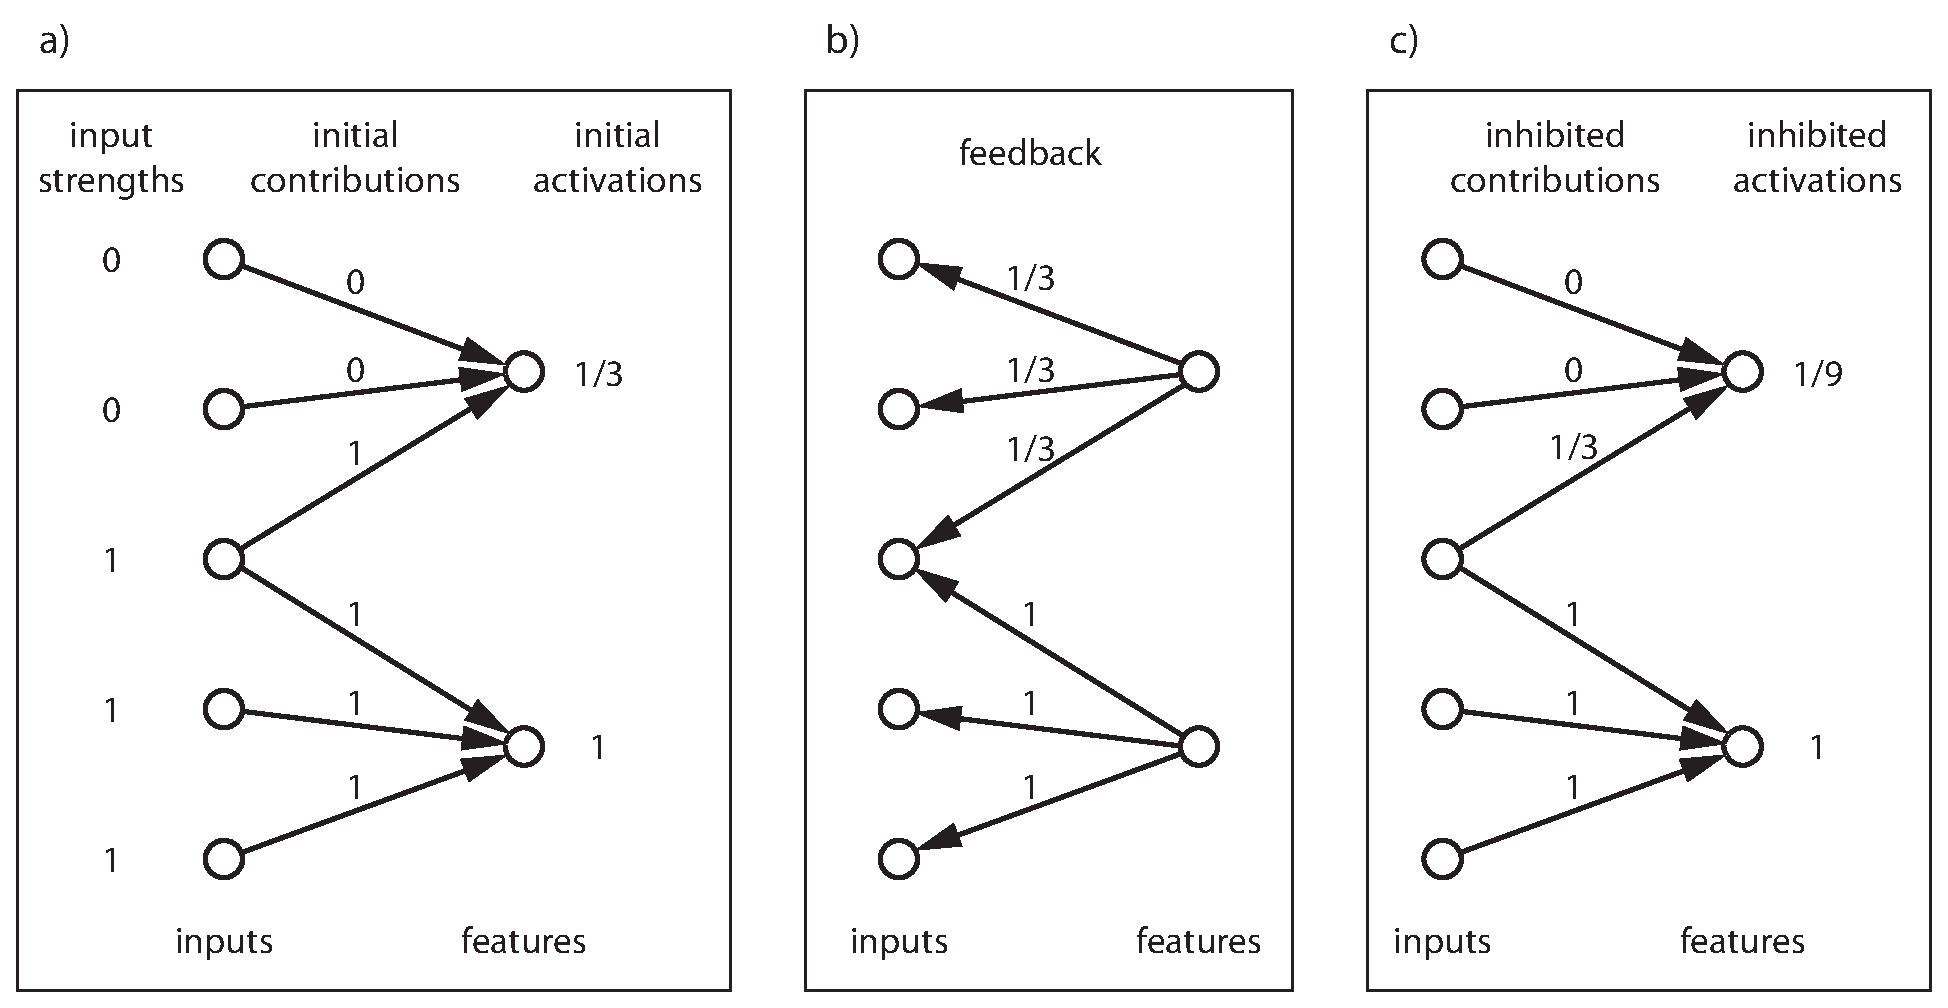
\includegraphics[height=7cm]{figs/competitive_activation.eps}
\caption{An example of competitive feature activation. {\bf a)} Inputs activate the features to their initial activity levels, $\hat{\mathbf{f}}$. {\bf b)} The $\hat{\mathbf{f}}$ values are fed back to the inputs. The feature with the highest $\hat{\mathbf{f}}$ for a given input suppresses that input's contributions to all other features. {\bf c)} As a result of this suppression (with $C_{awe} = 1$ in Equation~\ref{feedback_calculation}), the final activities, $\mathbf{f}$, of competing features are weakened.}
\label{competitive_activation}
\end{figure}

To be more precise, feature activities interact as follows. For an input that contributes to several different features, its contribution to feature $i$ will be inhibited by $\gamma_i$, given by:

\begin{equation}
\gamma_i = \left( \frac{\hat{f}_i}{\hat{f}_{\max}}\right ) ^ {C_{awe}}
\label{feedback_calculation}
\end{equation}

This formulation weakens all the contributions of the input except for the one to the most active feature, the one with $\hat{f}_{\max}$.

\subsection{Input energy}

The input magnitudes used to calculate co-activity can be lower than the original input magnitudes. Conceptually this is analogous to inputs having limited energy. If an input excites a feature strongly, then it has less energy available to build up new features with other inputs. But if an input excites no features, then it has plenty of energy available to establish co-activity with other inputs.

The fraction of its magnitude that an input devotes to co-activity is given by $\gamma_\kappa$:

\begin{equation}
\gamma_\kappa = 2 ^ { - C_{dif}\sum \gamma_i}
\end{equation}

When an input excites more features, $\sum \gamma_i$ gets larger, forcing $\gamma_\kappa$ smaller. This in effect creates a soft limit on the number of features an input can contribute to. 

\section{Hierarchy, time, and domain knowledge} 

Three additional details of \textsc{Becca}'s operation are necessary to achieve its full capabilities. 

\begin{enumerate}

\item The first of these is the recurrent handling of its inputs and outputs. In addition to being \textsc{Becca}'s output, the feature activities at each time step are fed back into the grouper as the next time step's inputs. This allows features to be grouped with each other and other inputs to form new groups, in which higher-level features will be created. Due to its recurrent structure, this process may be repeated indefinitely, creating a hierarchical feature structure with an arbitrarily large number of hierarchy levels. In practice, new groups are only formed as often as co-activity dictates, which is limited by the structure inherent in the data.

\item The second detail is the temporal decay of inputs. After an input is active, its channel retains some residual activity on subsequent time steps, even if it is not externally stimulated. This decay is of a geometric nature, resulting in an exponential decay curve: 

\begin{equation}
s_{k_{t+1}} = C_{idr} s_{k_t} \mbox{,   \hspace{0.2in}  } 0 < C_{idr} < 1
\end{equation}

The result of this decay is that temporal aspects of data can be captured in the features. For instance, if input $b$ is always active following input $a$, but never at the same time, retaining a decayed ghost of $a$'s activity allows it to be correctly correlated with that of $b$ to form a feature with temporal structure.

\item The third detail is the direct injection of user-created features to capture domain knowledge. As presented so far, \textsc{Becca} insists of deriving its own representation of the data from scratch. But in most applications, designers already have a pretty good guess about which features are likely to be informative in solving a given problem. \textsc{Becca} has a mechanism for incorporating engineered features as well. It looks for a vector of user-created feature primitives at each time step, in addition to raw sensor data. It handles the primitives differently that other inputs, concatenating them with the feature activities of all the created groups. As such, the primitives are both fed back as inputs, and included with the feature extractor's output. The only constraint on primitives is that they also be real valued between zero and one. \textsc{Becca} handles both raw sensor inputs and feature primitives as fuzzy binary inputs, each indicating the graded presence of a certain attribute.

\end{enumerate}


\section{Co-activity}
\label{coactivity_calc}
\textsc{Becca}'s co-activity calculation is incremental, with the update method for real valued inputs given by the following:

\begin{equation}
\Delta\kappa(a, b) = C_{pur} s_a ( s_a s_b - \kappa(a, b) ) \mbox{,  \hspace{0.2in}  } 0 < C_{pur} < 1		
\label{coactivity_update}
\end{equation}

Where $\kappa$ is the co-activity, and $s_a$ and $s_b$ are the activity levels of channels $a$ and $b$ respectively. For values of $s_a$ and $s_b$ that remain constant over time, a convergence value for $\kappa(a, b)$ can be found from Equation~\ref{coactivity_update}. For the convergence criteria to be met, $\Delta\kappa(a, b) = 0$. That implies $s_a s_b - \kappa(a, b) = 0$ (assuming $s_a > 0$), giving the steady state value of

\begin{equation}
\kappa(a, b) = s_a s_b 
\end{equation}

The steady state value is symmetric in $s_a$ and $s_b$, even though the update rule is not. For constant-valued $s_a$ and $s_b$, $\kappa(a, b)$ and $\kappa(b, a)$ converge to the same value, but at different rates. 

Another instructive case is that of binary and stochastic inputs. Consider the independent input channels $a$ and $b$ such that

\begin{eqnarray}
a &|& p(s_a = 1) = 0.5 \mbox{, \hspace{0.2in}  } p(s_a = 0) = 0.5\\
b &|& p(s_b = 1) = 0.1 \mbox{, \hspace{0.2in}  } p(s_b = 0) = 0.9 	
\end{eqnarray}

The structure of the update rule guarantees that $\Delta\kappa(a, b) = 0$ when $s_a = 0$ , meaning that $\kappa(a, b)$ will not be modified in any way. It will only be updated when $s_a = 1$. The steady state value for $\kappa(a, b)$ can then be calculated by observing that when $s_a = 1$ the update rule reduces to 

\begin{equation}
\Delta \kappa(a, b) = s_b - \kappa(a, b)  
\end{equation}

The fact that $b$ is independent from $a$ implies that $\kappa(a, b)$ will converge to the mean of $s_b=0.1$. Following a similar set of calculations, it can be shown that $\kappa(b, a)$ converges to 0.5 . This illustrates the effect of asymmetry in the update rule on non-constant input values. The results can be verbalized as ``Channel $a$ is co-active with Channel $b$ ten percent of the time, but Channel $b$ is co-active with Channel $a$ fifty percent of the time." An intuitive metaphor is that of restless kindergarteners at nap time. The teacher has told all the children to lay still and close their eyes, but unable to help themselves, some of the children occasionally peek. $\kappa(a, b)$ is the probability that, when child a peeks, she will see child b's eyes open and vice versa.

One final observation about $\kappa(a, b)$ is that it is bounded both above and below by the product of $s_a$ and $s_b$. Since $0 \leq s_a \leq 1$ and $0 \leq s_b \leq 1$ ,  it follows that 

\begin{eqnarray}
0 \leq&s_a s_b&  \leq 1 \\
0 \leq&\kappa(a, b)&  \leq 1 
\end{eqnarray}


\section{Constant values}

The values of the constants used in this version of \textsc{Becca} are listed in Table~\ref{perceiver_constants}. Its performance is quite sensitive to some of them, unfortunately. Eliminating these constants where possible is one of the secondary goals of development. Where elimination isn't possible, I try to find formulations that are insensitive to small changes in constants or combinations of values that work across a broad set of tasks and conditions.

\begin{table}[htdp]
\caption{Values used for feature extractor constants.}
\begin{center}
\begin{tabular}{|l|c|l|}
\hline
constant & value & description\\
\hline
$C_{sdr}$ & $10^{-3}$ & sensor distribution update rate \\
$C_{sut}$ & 5 & sensor update time constant \\
$C_{sim}$ & 0 & sensor initial mean \\
$C_{sid}$ & 0.01 & sensor initial deviation \\
$C_{nft}$ & 0.1 & new feature threshold \\
$C_{msc}$ & 0.07 & minimum significant co-activity threshold \\
$C_{awe}$ & 10 & activation weighting exponent \\
$C_{dif}$ & 0.3 & dissipation factor \\
$C_{idr}$ & 1.0 & input decay rate \\
$C_{pur}$ & $10^{-3}$ & plasticity update rate \\
\hline
\end{tabular}
\end{center}
\label{perceiver_constants}
\end{table}%

